\chapter{Исследовательская часть}

В данном разделе будут приведены примеры работы программы, а также проведен сравнительный анализ процессорного времени работы реализаций алгоритмов при различных ситуациях на основе полученных данных.

\section{Технические характеристики}

Технические характеристики устройства, на котором выполнялись замеры времени представлены далее:

\begin{itemize}
	\item операционная система Windows 11 Pro Версия 22H2 (22621.674) \cite{wind};
	\item память 16 ГБ;
	\item процессор 11th Gen Intel(R) Core(TM) i5-11400 2.59 ГГц \cite{proc}.
\end{itemize}

При тестировании компьютер был включен в сеть электропитания. Во время замеров процессорного времени устройство было нагружено только встроенными приложениями окружения, а также системой тестирования.

\section{Демонстрация работы программы}

На рисунке \ref{img:res} представлен результат работы программы. На экран выводятся результаты заемров времени для разных размеров строк и разных видов алгоритмов поиска расстояний Левенштейна и Дамерау-Левенштейна в мс.
\newpage
%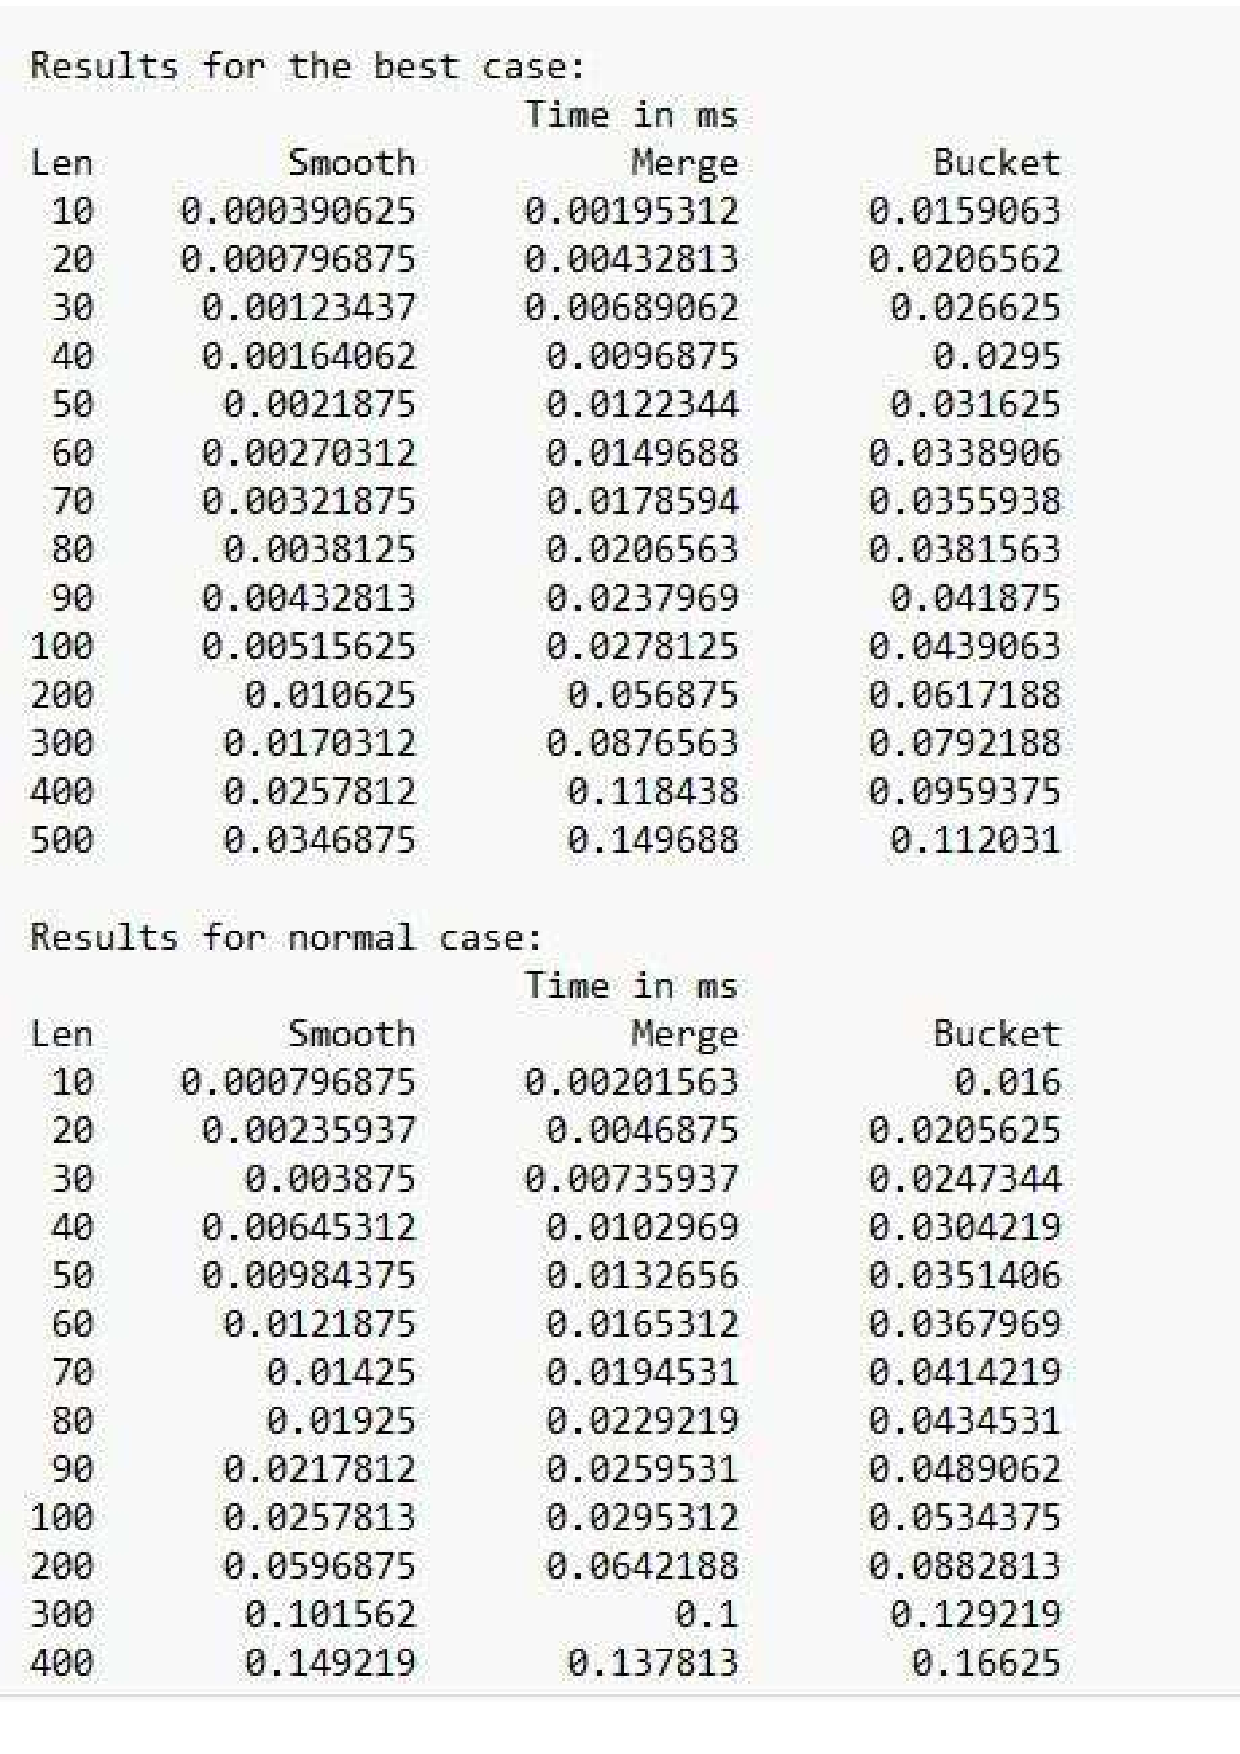
\includepdf[pages=-]{src/screen.pdf}
\begin{center}
	\centering{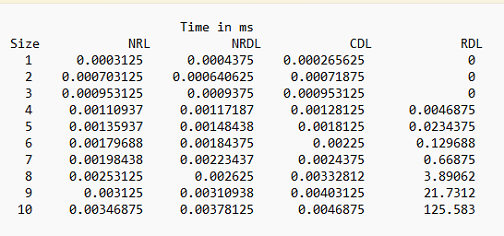
\includegraphics[trim=0 0 0cm 0cm bb=0 0 504 320]{src/screen}}
	\captionof{figure}{Пример работы программы}
	\label{img:res}
\end{center}

\section{Время выполнения реализаций алгоритмов}

Как было сказано выше, используется функция замера процессорного времени GetProcessTimes(...) из библиотеки Windows.h. 

\textbf{Входные данные:} строки размером от 1 до 10 символов для сравнений рекурсивной версии алгоритма поиска расстояния Дамерау-Левенштейна и остальных алгоритмов; строки размером от 10 до 500 символов для остальных случаев сравнения.

Результаты замеров времени работы реализаций алгоритмов поиска расстояний Левенштейна и Дамерау-Левенштейна на различных входных данных (в мс) приведены в таблицах \ref{tbl:best}, \ref{tbl:best1}.
\begin{center}
	\begin{threeparttable}
		\caption{Процессорное время работы реализаций алгоритмов на малом размере входных строк}
		\label{tbl:best}
		\begin{tabular}{|c|c|c|c|c|}
			\hline
			Размер &р. Л.(матр.) &р. Д-Л.(матр.)  &р. Д-Л.(рек. с кешем)& р. Д-Л.(рек.)\\
			\hline
			1 &  0.0003125  &    0.0004375    &0.000265625 &             0\\
			\hline
			2 &  0.000703125 &   0.000640625    & 0.00071875&              0\\
		\hline
			3 &  0.000953125  &    0.0009375   & 0.000953125 &             0\\
		\hline
			4 & 0.00110937     &0.00117187    & 0.00128125    &  0.0046875\\
		\hline
			5 &  0.00135937     &0.00148438      &0.0018125    &  0.0234375\\
		\hline
			6 & 0.00179688 &    0.00184375      &  0.00225      & 0.129688\\
		\hline
			7 &  0.00198438 &    0.00223437    &  0.0024375      &  0.66875\\
		\hline
			8 & 0.00253125   &    0.002625    & 0.00332812        &3.89062\\
		\hline
			9 & 0.003125 &    0.00310938     &0.00403125      &  21.7312\\
		\hline
			10 & 0.00346875 &    0.00378125 &     0.0046875    &    125.583\\
		\hline
		\end{tabular}
		
	\end{threeparttable}
\end{center}

\begin{center}
	\begin{threeparttable}
		\caption{Процессорное время работы реализаций алгоритмов на большом размере входных строк}
		\label{tbl:best1}
		\begin{tabular}{|c|c|c|c|}
			\hline
			Размер &р. Л.(матр.) &р. Д-Л.(матр.)  &р. Д-Л.(рек. с кешем)\\
			\hline
		 	10  &     0.003125     &         0   &     0.00625 \\
			\hline
			 20   &      0.0125   &     0.00625   &    0.015625 \\
			\hline
			30   &     0.00625   &    0.021875    &   0.034375  \\
			\hline
			40   &    0.021875  &     0.040625    &   0.028125\\
			\hline
			50    &   0.053125  &     0.065625   &     0.09375\\
			\hline
		 	60   &    0.084375  &     0.059375   &      0.1375\\
			\hline
			70    &   0.096875   &     0.10625    &    0.19375 \\
			\hline
			80    &   0.146875    &    0.15625    &     0.2125\\
			\hline
			 90   &    0.184375   &    0.178125   &      0.3125\\
			\hline
			100    &   0.196875   &    0.228125   &         0.4\\
			\hline
			200   &     0.85625    &      0.925   &     1.58125\\
			\hline
			300   &     1.88437    &          2   &         3.5\\
			\hline
			400    &    3.40937     &    3.5875   &     6.34063\\
			\hline
			500     &   5.40313     &   5.59687    &     9.7375\\
			\hline
		\end{tabular}
		
	\end{threeparttable}
\end{center}
Также на рисунках \ref{img:graph_sorted},  \ref{img:graph_sorted1}, \ref{img:graph_sorted2} приведены графические результаты замеров времени работы алгоритмов в зависимости от линейного размера входных строк.

\begin{center}
	\centering{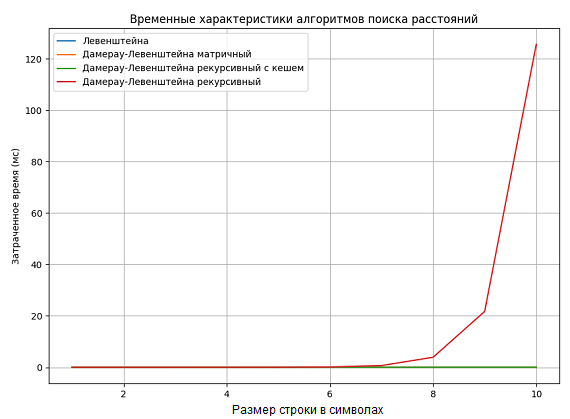
\includegraphics[trim=0 0 0 -5cm bb=0 0 570 650]{src/Graph}}
	\captionof{figure}{Процессорное время вычислений}
	\label{img:graph_sorted}
\end{center}

\begin{center}
	\centering{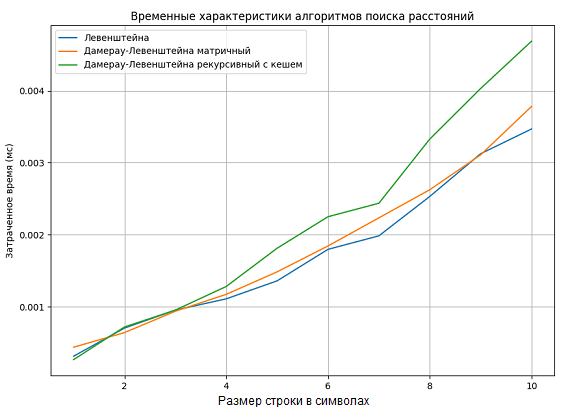
\includegraphics[trim=0 0 0 -5cm bb=0 0 570 650]{src/Graph1}}
	\captionof{figure}{Процессорное время вычислений}
	\label{img:graph_sorted1}
\end{center}

\begin{center}
	\centering{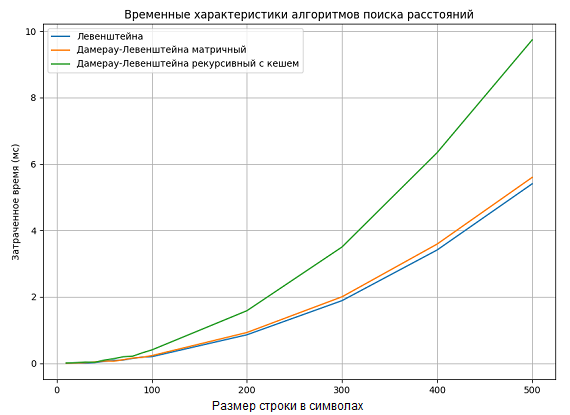
\includegraphics[trim=0 0 0 -5cm bb=0 0 570 650]{src/Graph2}}
	\captionof{figure}{Процессорное время вычислений}
	\label{img:graph_sorted2}
\end{center}
\newpage

\section{Вывод}
По полученным результатам ислледования можно сделать вывод, что рекурсивные реализации поиска расстояний Дамерау-Левенштейна работают гораздо дольше по времени в отличии от матричных реализаций того же алгоритма и алгоритма поиска расстояния Левенштейна: в 41666 и 1.3 раза для рекурсивного и рекурсивного с кешированием соответственно. Таким образом наличие кеша снижает временные затраты на рекурсивный алгоритм в 31000 раз. 
